\section{Introduction}
The coronavirus pandemic has hit hard most of the world's countries in the last two years, with the latest variation, Omicron, proving to be a very contagious one.
One of the main protection measures countries have taken against the pandemic is the provision of newly developed vaccines for the general population. However, after getting vaccinated against COVID-19, protection against the virus and the ability to prevent infection with variants may decrease over time and due to changes in variants. This is why additional booster shots have also been introduced to further protect the public from infection.
\\
In this report, we perform an analysis of vaccination world data for the novel coronavirus (COVID-19) using the R language in order to extract useful information on the data on a country, continent or world level.

\subsection{Dataset}
The dataset utilized in this report is taken directly from a 
\href{https://cran.r-project.org/web/packages/coronavirus/coronavirus.pdf}{C-RAN project}, and contains a daily summary of the COVID-19 vaccination by country / province.
The vaccine data source of the dataset is Johns Hopkins University Centers for Civic Impact (JHU CCSE) COVID-19 \href{https://github.com/govex/COVID-19}{repository}.

\subsection{R packages}

% define formatting of R code
\newtcblisting{Rcode}[1]{
  listing engine=minted,
  colback=code_bg,
  colframe=black!70,
  listing only,
  minted style=colorful,
  minted language=R,
  minted options={fontsize=#1, texcl=true},
  left=1mm,
  fonttitle=\bfseries
}
\definecolor{code_bg}{rgb}{0.85,0.85,0.85}

The two main R language packages used in this report are the following:

\begin{center}
    \begin{tabular}{ |c|c|c| } 
     \hline
     data.table & R package used for working with tabular data \\
     \hline 
     ggplot2 & R package dedicated to data visualization \\ 
     \hline
    \end{tabular}
\end{center}

Below is the code with all the packages used:
\begin{Rcode}{\scriptsize}
# Include packages
library(coronavirus) # coronavirus package
library(ggplot2) # data vizualizations/plots
library(treemapify) # use with ggplot2 for treemaps
library(ggpubr) # combine ggplot2 plots in multiple rows/cols
library(data.table) # working with tabular data
library(scales) # used for custom scaling on ggplot axes
\end{Rcode}


\section{Load Data}
\subsection{Read the data}
First we load the data in a data table from a downloaded csv file "covid19\_vaccine.csv".
\\
The last update of the data was on \textbf{08-01-2022}.

\begin{Rcode}{\scriptsize}
#set env language to English (eg date in plots to be shown in English)
Sys.setenv("LANGUAGE"="En")
Sys.setlocale("LC_ALL", "English")

# Read the vaccinations dataset
DT = fread("covid19_vaccine.csv", data.table = TRUE) #load data in data table
is.data.table(DT)
\end{Rcode}
[1] TRUE

\subsection{Data inspection}
In this section, we inspect the data loaded in the data table from the csv dataset file.
\\ \\
\textbf{\# columns}: 18
\\
\textbf{\# rows}: 143,629
\\
\textbf{last day with data}: 08-01-2022
\\
\textbf{first day with data}: 14-12-2020
\\
\textbf{date difference last-first+1 day}: 391 days
\\
\textbf{\# of countries}: 190 (+world as an extra entry with aggregate data)

\begin{Rcode}{\scriptsize}
# Examine the vaccination dataset
head(DT) #inspect the dataframe's first few lines
#check the length of the dataframe (number of columns) = 18
initial_columns_number = length(DT)
#check the length of one of the columns => (number of rows) = 143629
dataset_rows_number = length(DT$date) 

end_date = max(DT$date) # last day for which data are available = 08-01-2022
start_date = min(DT$date) # first day for which data is available = 14-12-2020
# number of days for which we have data = 391 days
days_covered_in_dataset = end_date - start_date + 1 
# unique country regions = 191 (actual number  190 as "World" is included)
unique_country_regions = DT[, length(unique(country_region))] 
\end{Rcode}
\\
In \textbf{Figure \ref{fig:dataset_inspection}} is a snippet of the dataset for the first few days recorded.
We can see that there are no available data for each country for each day. For instance, on 14-12-2020 there is only data available for Canada and World and on 15-12-2020 for Canada, China, Russia and World.

% data from initial data table
\begin{figure}[h]
    \centering
    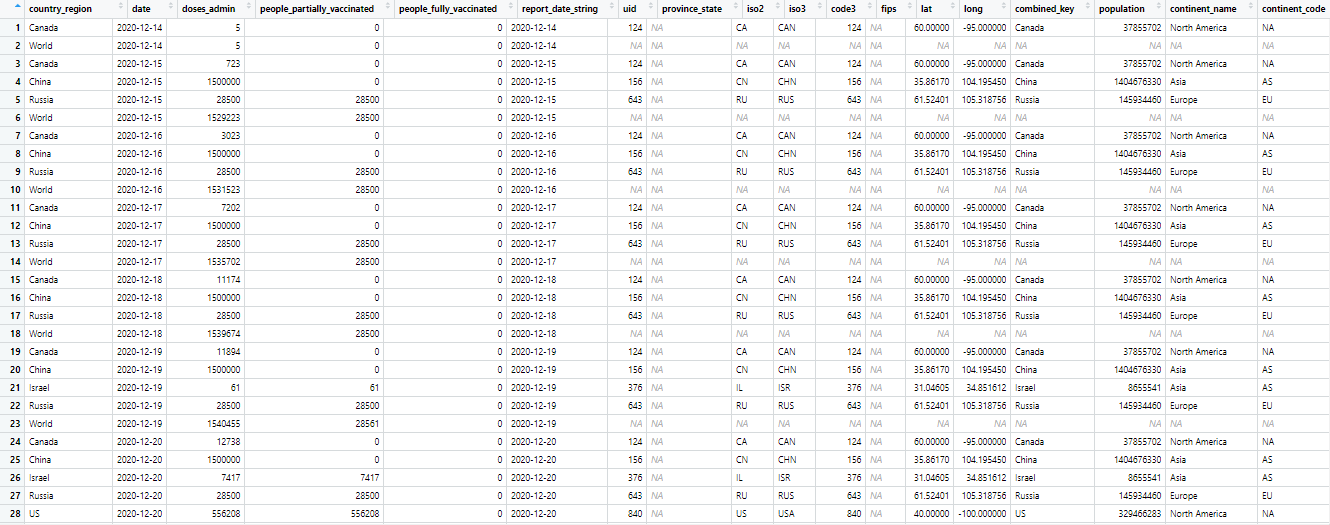
\includegraphics[width=15cm,height=\textwidth, left, keepaspectratio]{figures/DT - overview of initial data.PNG}
    \caption{Inspection of first few lines of the dataset}
    \label{fig:dataset_inspection}
\end{figure}
\FloatBarrier %fix position of image to its own subsection, not the next

\section{Data processing}
In this section of the report, data is processed and manipulated in order to clean data, construct new useful variables, and overall prepare data for the subsequent exploratory data analysis.
The 18 columns of the initial dataset are in the following \textbf{Table \ref{tab:columns_table}}.

% description of the 18 columns of the dataset
\begin{table}[h]
\small
\begin{tabular}{l|p{70mm}}
     \hline
     country\_region & Country or region name \\
     date & Data collection date in YYYY-MM-DD format \\ 
     doses\_admin & Cumulative number of doses administered \\
     people\_partially\_vaccinated & Cumulative number of people who received at least one vaccine dose \\
     people\_fully\_vaccinated & Cumulative number of people who received all prescribed doses necessary to be considered fully vaccinated \\
     report\_date\_string & Data report date in YYYY-MM-DD format \\
     uid & Country code \\
     province\_state & Province or state if applicable \\
     iso2 & Officially assigned country code identifiers with two-letter \\
     iso3 & Officially assigned country code identifiers with three-letter \\
     code3 & UN country code \\
     fips & Federal Information Processing Standards code that uniquely identifies counties within the
     USA \\
     lat & Latitude \\
     long & Longitude \\
     combined\_key & Country and province (if applicable) \\
     population & Country or province population \\
     continent\_name & Continent name \\
     continent\_code & Continent code \\
     \hline
\end{tabular}
\caption{\label{tab:columns_table}Columns of initial dataset \& description}
\end{table}

\subsection{New variables}
Two new variables are firstly created by dividing the values of the variables people\_fully\_vaccinated and people\_partially\_vaccinated respectively by the values of the variable population. The two new variables created are the following: \\ \\
\textbf{fully\_vaccinated\_ratio}
\\
\textbf{partially\_vaccinated\_ratio}
\\ \\
Moreover, the relative frequencies are converted to percentages keeping one decimal place.

\begin{Rcode}{\scriptsize}
# Update data table with fully\_vaccinated\_ratio column (percentage, 1 decimal digit)
DT = DT[, fully_vaccinated_ratio := round(100 * 
(people_fully_vaccinated / population), digits = 1)]

# And then with partially\_vaccinated\_ratio column
DT = DT[, partially_vaccinated_ratio := round(100 * 
(people_partially_vaccinated / population), digits = 1)]
\end{Rcode}


\subsection{Data removal}
Out of the initial 143,629 data rows in the dataset, the ones concerning provinces are removed, which is the majority of the data. We end up with 55,513 rows in the resulting dataset. \\
The removal happens by firstly filtering out all rows where the province\_state field is not NA (Not Assigned) or equally contains some value (province or state). Then, the column province\_state is dropped from the data table.

\begin{Rcode}{\scriptsize}
# Keep only country & world data - keep rows with NA value under province\_state
# Those are the aggregate values for each country

# Filter out province\_state values that are not NA (ie referring to provinces)
DT = DT[is.na(province_state)] 
DT = DT[, province_state:=NULL] # Remove province\_state column from datatable 
\end{Rcode}
\\

\subsection{Data cleaning}
Additionally, some data are corrupted and therefore are fixed in order for the subsequent data analysis to be more accurate. \\
Initially, data rows with partially\_vaccinated\_ratio or fully\_vaccinated\_ratio value over 100\% are obviously wrong and should be fixed. The handling in these cases was to adjust the ratio down to 100\%. 

\begin{Rcode}{\scriptsize}
#returns rows indices of DT that fully vaccinated ratio exceeds 100%
which(DT[,fully_vaccinated_ratio]>100)
\end{Rcode}
\textbf{result:} integer(0)
\\
This means there are no rows with fully\_vaccinated\_ratio over 100\%

\begin{Rcode}{\scriptsize}
#returns rows indices of DT that partially vaccinated ratio exceeds 100
which(DT[,partially_vaccinated_ratio]>100)  
\end{Rcode}
[1] 34019 34183 35003 53520 53711 53902 54093 54284 54475 54666 54857 55048 55239 55430
\\
There are 14 rows out of the 55,513 of the data table that have partially\_vaccinated\_ratio over 100\% and those are adjusted to 100\%.

\begin{Rcode}{\scriptsize}
#check max value is now 100%
DT[partially_vaccinated_ratio > 0, max(partially_vaccinated_ratio)]
\end{Rcode}
[1] 100
\\
With the previous command it is verified that the partially\_vaccinated\_ratio column contains values up to 100\%.
\\
Another data cleaning task was to identify rows with missing continent\_name values that will be used in the data analysis.

\begin{Rcode}{\scriptsize}
# Find missing continent values
DT[is.na(continent_name) & country_region != 'World', unique(country_region)]
\end{Rcode}
[1] "Sudan"  "Kosovo"
\\
The above result means that rows with country\_region values of Sudan or Kosovo have missing continent\_name value. Therefore there is a need to fill in those values with their appropriate name of the continent they belong to.

\begin{Rcode}{\scriptsize}
# Fix missing continent values
which(DT[, country_region]=='Kosovo')
#set continent name for Kosovo to Europe
set(DT, i=which(DT[, country_region]=='Kosovo'), j=16L, value='Europe') 
#set continent code for Kosovo to EU
set(DT, i=which(DT[, country_region]=='Kosovo'), j=17L, value='EU') 
which(DT[, country_region]=='Sudan')
#set continent name for Sudan to Africa
set(DT, i=which(DT[, country_region]=='Sudan'), j=16L, value='Africa') 
#set continent code for Sudan to AF
set(DT, i=which(DT[, country_region]=='Sudan'), j=17L, value='AF') 
\end{Rcode}
The datatable rows have been updated after the last step.

\section{Exploratory Data Analysis}
This is the main section of the report, containing data manipulations and graphical representations of the data in order to extract useful information from the dataset.

\subsection{World vaccination progress}
First we draw the cumulative number of people who received at least one vaccine dose on a global level over time. For this, the people\_partially\_vaccinated variable was used.

\begin{Rcode}{\scriptsize}
# People partially vaccinated progress - World
world_partial_data = DT[country_region == 'World', 
                        .(date, people_partially_vaccinated)]

partially_vacc_worldwide <-  
  ggplot(world_partial_data, aes(x=date)) +
  geom_area(aes(y=people_partially_vaccinated), alpha=0.5) +
  labs(title="World - Number of people partially vaccinated",
       subtitle="Vaccination progress on a global scale",
       x="Date", 
       y="People partially vaccinated") +
  theme(axis.text.x = element_text(angle=45)) + 
  scale_x_date(date_breaks = "1 month", date_labels = "%b %Y") +
  scale_y_continuous(labels = unit_format(unit = "Billions", scale = 1e-9))

partially_vacc_worldwide
\end{Rcode}

\begin{figure}[h]
    \centering
    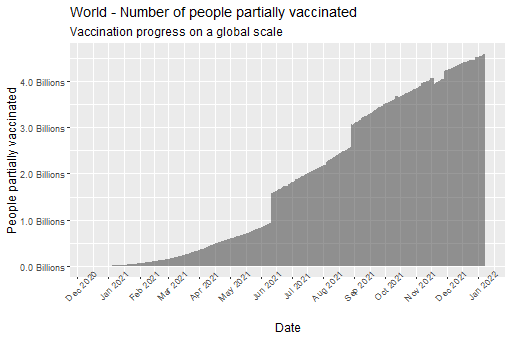
\includegraphics[height=7cm]{figures/World-people partially vaccinated progress over time.png}
    \caption{Progress of cumulative number of people receiving at least one vaccine dose worldwide}
    \label{fig:world_people_progress}
\end{figure}
\FloatBarrier %fix position of image to its own subsection, not the next

From \textbf{Figure \ref{fig:world_people_progress}}, it comes that approximately 5 billion people had received at least one vaccine dose by 08-01-2022. This is around 60\% of the global population as illustrated also in \textbf{Figure \ref{fig:world_ratios_progress}}.
Also, another observation here is that vaccinations started at the beginning of 2021 and ramped up around June 2021 and then again on September 2021.

\begin{Rcode}{\scriptsize}
world_data = DT[country_region == 'World'] #World data by date
#keep 1 row for each country -> contains eg its population
countries_info = unique(DT, by=c('country_region')) 
# world\_population=7.331.618.789, slightly above real value (~7.9 billion)
world_population = countries_info[country_region != 'World', 
                                sum(population, na.rm=TRUE)] 

x <- ggplot(world_data, aes(x=date)) +
  geom_line(aes(y=round(100*people_partially_vaccinated/world_population,digits=1), 
                colour = 'Partially vaccinated'), size = 1) +
  geom_line(aes(y=round(100*people_fully_vaccinated/world_population, digits=1), 
                colour = 'Fully vaccinated'), size = 1) +
  scale_color_manual(name = "Legend", 
                     values = c("Partially vaccinated" = "darkblue", 
                     "Fully vaccinated" = "red")) +
  labs(title = 'World - Vaccination ratios',
       subtitle='Vaccination progress on a global scale',
       y = 'Vaccination ratios',
       x = 'Date') +
  scale_x_date(date_breaks = "1 month", date_labels = "%b %Y") +
  theme(axis.text.x = element_text(angle=45, hjust = 1)) +
  scale_y_continuous(labels = unit_format(unit = "%"))

x #display plot in RStudio
\end{Rcode}

\begin{figure}[h]
    \centering
    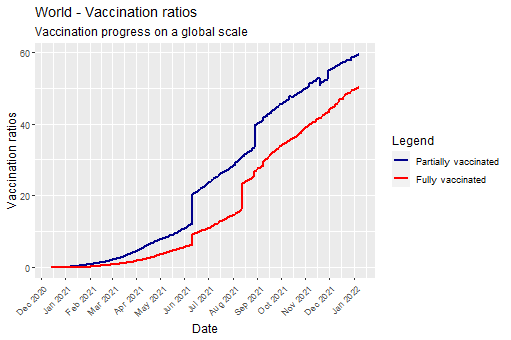
\includegraphics[width=12cm]{figures/World - vacc ratios (partially & fully).png}
    \caption{Progress of cumulative vaccination ratios worldwide}
    \label{fig:world_ratios_progress}
\end{figure}
\FloatBarrier %fix position of image to its own subsection, not the next

In \textbf{Figure \ref{fig:world_ratios_progress}} one can see that as expected, the fully vaccinated ratio is always below the partially vaccinated ratio and it's maximum value has reached around 50\%. Also, there is a big ramp up in the fully vaccinated ratio in mid-August 2021 given that 2nd vaccination doses were generally administered depending on the vaccine a few weeks after the first one and there was a ramp up on partial vaccinations earlier in the summer.
\\
Next, a treemap of partially and fully vaccinated ratio is presented where the tiles size corresponds to the country's population and color brighness is proportional to the level of vaccination ratio.

\begin{Rcode}{\scriptsize}
#data of the last day recorded (exclude World aggregate data)
last_day_data = DT[date == "2022-01-08" & country_region != 'World'] 
treemap1 = ggplot(last_day_data, aes(area = population, 
                  fill = partially_vaccinated_ratio, label = country_region)) +
  labs(title='Treemap of partially vaccinated ratio per country population',
       subtitle='Size of tile: population, Date = 08-01-2022', fill='Ratio %') +
  geom_treemap() + geom_treemap_text(colour = "white",place = "centre")
treemap2 = ggplot(last_day_data, aes(area = population,
                  fill = fully_vaccinated_ratio, label = country_region)) +
  labs(title='Treemap of fully vaccinated ratio per country population',
       subtitle='Size of tile: population, Date = 08-01-2022', fill='Ratio %') +
  geom_treemap() + geom_treemap_text(colour = "white", place = "centre") 

# combine both treemaps in a single figure
figure <- ggarrange(treemap1, treemap2, ncol = 1, nrow = 2) #combine two ggplots
figure
\end{Rcode}

\begin{figure}[h]
    \centering
    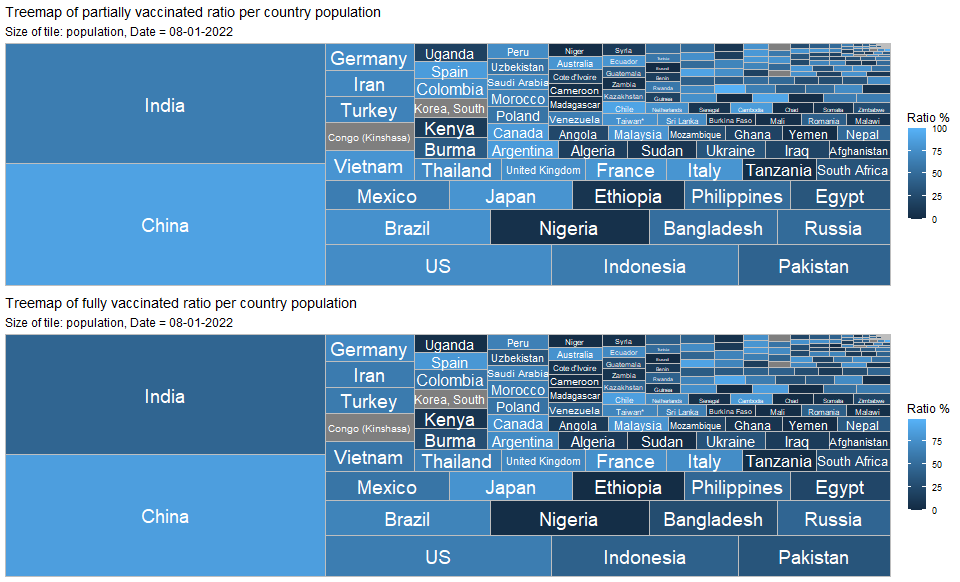
\includegraphics[width=12cm, height=8cm]{figures/Treemap - all countries (fully and partially).png}
    \caption{Treemap of vaccination ratios by country population}
    \label{fig:world_ratios_treemap}
\end{figure}
\FloatBarrier %fix position of image to its own subsection, not the next

The first observation from \textbf{Figure \ref{fig:world_ratios_treemap}} is that partially vaccinated ratios and fully ones give almost the same information on a country level since the two treemaps are almost identical.
\\
Another observation is that African countries such as Nigeria, Ethiopia, Tanzania, Kenya and others are lacking behind in terms of the vaccination ratios (both partially and fully ones) compared to the countries of other continents.
\\
China, despite its large population have managed to perform very well in terms of vaccination rates. Poorer Asian countries such as India, Indonesia, Pakistan, Bangladesh and others, however, have not managed to achieve high rates. Also, it's pretty obvious that European countries have in general performed well given their bright colors.
\\
Another observation has to do with the data quality. There are missing values for the two ratios (eg Congo, South Korea and others) denoted with gray colored tiles in the treemaps, which is a result of missing values for the people\_partially\_vaccinated and people\_fully\_vaccinated columns of the data for those countries.

\subsection{Top vaccinated countries}
Next, we analyse and compare the countries with the top vaccination ratios and explore whether the largest countries in terms of population are also leaders in vaccination rates. \\
Initially, a bar plot is created for the top 20 most populated countries and their partially vaccinated ratios. Please note, that the focus of the report moving forward will be on partially vaccinated ratios over fully ones given their overall parallel trajectory.

\begin{Rcode}{\scriptsize}
last_day_data_top_20_population = last_day_data[order(-population)]
last_day_data_top_20_population = last_day_data_top_20_population[1:20]

barplot3<-ggplot(data=last_day_data_top_20_population,
                 aes(x=reorder(country_region, partially_vaccinated_ratio), 
                     y=partially_vaccinated_ratio, fill=continent_name)) +
  geom_bar(stat='identity') +
  labs(
    title="Bar plot of 20 most populated countries' partially vaccinated ratios",
    subtitle='Date: 08-01-2022', fill='Continent',
    x='Country', y='partially vaccinated ratio %') +
  coord_flip() # Horizontal bar plot

barplot3
\end{Rcode}


\begin{figure}[h]
    \centering
    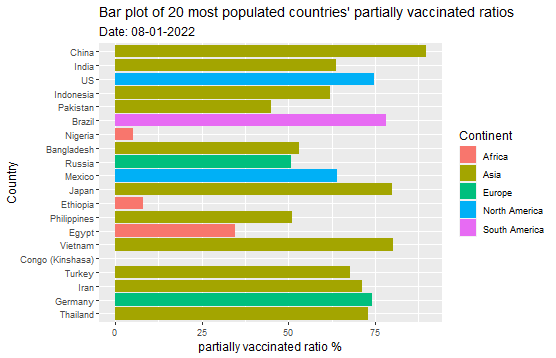
\includegraphics[width=12cm]{figures/Barplot_top20_population.png}
    \caption{Barplot of partially vaccination ratios of top 20 most-populated countries}
    \label{fig:top_20_population}
\end{figure}

Data on the vertical axis of \textbf{Figure \ref{fig:top_20_population}} is in descending order based on the population (largest to smallest). As illustrated from this figure as well, China is one of the leaders in vaccination rates, whereas the rest of the Asian countries that are highly populated are following. African countries are clearly lacking behind.
\\
Since that figure was dominated by Asian countries, a bar plot of the top 20 countries in terms of vaccination rates follows.

\begin{Rcode}{\scriptsize}
last_day_data_top_20_part_vacc_ratios = last_day_data[
                                        order(-partially_vaccinated_ratio)]
last_day_data_top_20_part_vacc_ratios = last_day_data_top_20_part_vacc_ratios[1:20]

barplot4<-ggplot(data=last_day_data_top_20_part_vacc_ratios, 
                 aes(x=reorder(country_region, partially_vaccinated_ratio), 
                     y=partially_vaccinated_ratio, fill=continent_name)) +
  labs(title="Bar plot of 20 top countries' partially vaccinated ratios",
       subtitle='Date: 08-01-2022', fill='Continent',
       x='Country', y='partially vaccinated ratio %') +
  geom_bar(stat='identity') +
  coord_flip() # Horizontal bar plot

barplot4
\end{Rcode}

Interestingly enough, from the resulting following \textbf{Figure \ref{fig:top_20_ratios}}, one can see that out of the top 20 countries in terms of the partially vaccination ratio, only China is in the 20 most populated countries. An assumption for the reason of this is that such countries face spacial, economical or other type of challenges in administering vaccination doses to the general public compared to smaller countries that have topped the chart.

\begin{figure}[h]
    \centering
    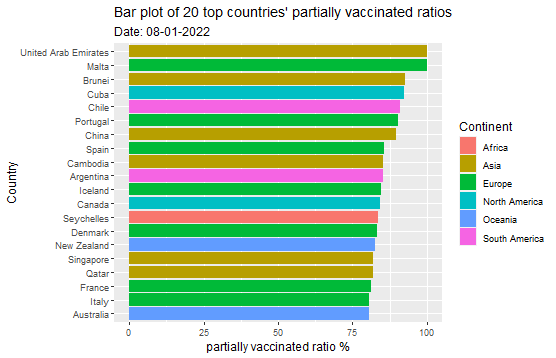
\includegraphics[width=12cm]{figures/Barplot_top20_vacc_ratios.png}
    \caption{Barplot of partially vaccination ratios of top 20 countries}
    \label{fig:top_20_ratios}
\end{figure}
\FloatBarrier %fix position of image to its own subsection, not the next

\subsection{Continent vaccination}
In this section, aggregated data concerning the 6 continents is presented.

\begin{Rcode}{\scriptsize}
#remove rows with NA partially\_vaccinated\_ratio
last_day_data_per_continent = na.omit(last_day_data, 
                                      cols="partially_vaccinated_ratio") 
last_day_data_per_continent = last_day_data_per_continent[, 
    .(population_total = as.double(sum(population)), 
    partially_vaccinated_ratio = round(100*sum(people_partially_vaccinated)/
                                         sum(population)),digits=1),
    by='continent_name']

treemap5 = ggplot(last_day_data_per_continent, aes(area = population_total, 
                fill = partially_vaccinated_ratio, label = continent_name)) +
  labs(title="Treemap of 6 continents' partially vaccinated ratios",
       subtitle='Tile size: population, Date: 08-01-2022', fill='Ratio %') +
  geom_treemap() +
  geom_treemap_text(colour = "white",
                    place = "centre")
barplot5<-ggplot(data=last_day_data_per_continent, 
                 aes(x=reorder(continent_name, partially_vaccinated_ratio), 
                 y=partially_vaccinated_ratio, fill=partially_vaccinated_ratio)) +
  labs(title="Bar plot of 6 continents' partially vaccinated ratios",
       subtitle='Date: 08-01-2022', fill='Ratio %',
       x='Country', y='partially vaccinated ratio %') +
  geom_bar(stat='identity') +
  coord_flip() # Horizontal bar plot
figure <- ggarrange(treemap5, barplot5, ncol = 1, nrow = 2) #combine two ggplots
figure
\end{Rcode}

\begin{figure}[h]
    \centering
    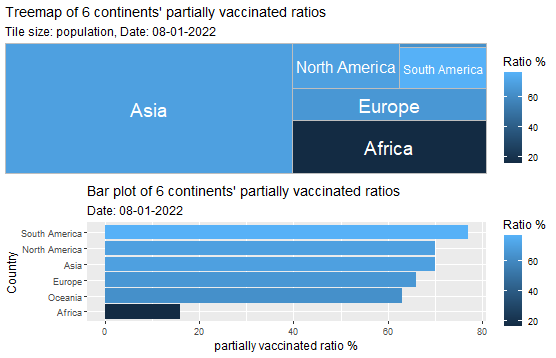
\includegraphics[width=12cm]{figures/Treemap_Barplot_Continents_ratios.png}
    \caption{Treemap \& Barplot of partially vaccination ratios of continents}
    \label{fig:continents_ratios}
\end{figure}
\FloatBarrier %fix position of image to its own subsection, not the next

From the presented  \textbf{Figure \ref{fig:continents_ratios}}, South America seems to be leading the partially vaccination ratio race with over 75\% with North America and Asia following with around 70\%. Europe is next with around 65\%, Oceania with around 62\% and, finally, Africa comes last with less than 20\%.

\subsection{African countries' vaccination ratios}
Given the very low ratio for the African continent, data from the continent is further explored for its countries to detect potential large differences among countries.

\begin{Rcode}{\scriptsize}
# explore African countries numbers on the last day of the dataset 08-01-2022
africa_last_day_data = DT[continent_name == 'Africa' & date == '2022-01-08']
# there are some countries with NA values
barplot6<-ggplot(data=africa_last_day_data, 
                   aes(x=reorder(country_region, partially_vaccinated_ratio), 
                       y=partially_vaccinated_ratio, 
                       fill=population)) +
  labs(title="Bar plot of African countries' partially vaccinated ratios",
       subtitle='Date: 08-01-2022', fill='Population',
       x='Country', y='partially vaccinated ratio %') +
  scale_fill_continuous(labels = unit_format(unit = "Millions", scale = 1e-6))+
  geom_bar(stat='identity') +
  coord_flip() # Horizontal bar plot
barplot6 #display the barplot
\end{Rcode}

\begin{figure}[h]
    \centering
    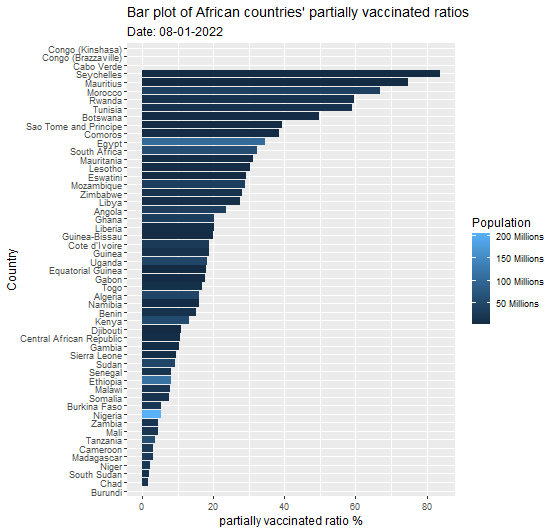
\includegraphics[width=12cm]{figures/Africa_ratios.png}
    \caption{Barplot of African countries' vaccination ratios}
    \label{fig:africa_ratios}
\end{figure}
\FloatBarrier %fix position of image to its own subsection, not the next

As shown on \textbf{Figure \ref{fig:africa_ratios}}, the majority of African countries have partially vaccinated ratios lower than 40\% on 08-01-2022. Also, the most populated ones have low ratios therefore dominating the continent's aggregated value.

\subsection{European countries' vaccination}
Next, we present the same bar plot for European countries.

\begin{Rcode}{\scriptsize}
last_day_data_Europe = last_day_data[continent_name == 'Europe']
barplot7<-ggplot(data=last_day_data_Europe,
                 aes(x=reorder(country_region, partially_vaccinated_ratio), 
                 y=partially_vaccinated_ratio, fill=population)) +
  labs(title="Bar plot of European countries' partially vaccinated ratios",
       subtitle='Date: 08-01-2022', fill='Population',
       x='Country', y='partially vaccinated ratio %') +
  scale_fill_continuous(labels = unit_format(unit = "Millions", scale = 1e-6))+
  geom_bar(stat='identity') + coord_flip() # Horizontal bar plot
barplot7
\end{Rcode}

\begin{figure}[h]
    \centering
    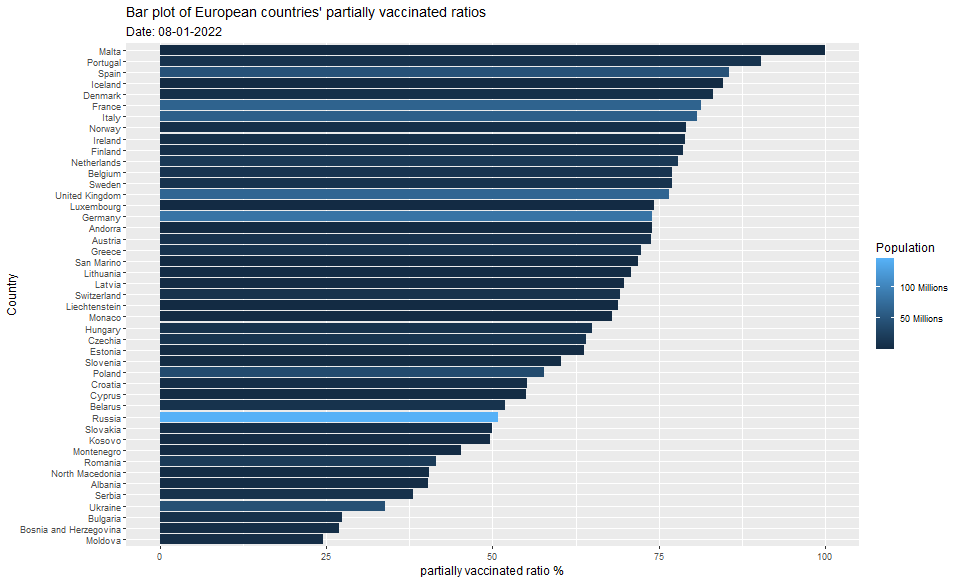
\includegraphics[width=12cm, height=10cm]{figures/Europe_ratios.png}
    \caption{Barplot of European countries' vaccination ratios}
    \label{fig:europe_ratios}
\end{figure}
\FloatBarrier %fix position of image to its own subsection, not the next

Interestingly, south Europe has topped the chart in the first 3 positions. Also, contrary to Africa, in Europe large countries have achieved high vaccination rates, better on average than smaller countries in the continent.

\subsection{Greece vaccination}
Finally, the partially vaccinated ratio of Greece is examined compared to average of the rest of Europe and the average of the rest of Balkans over time to get a sense of the country's performance versus the average of other countries in the European and Balkans regions.


\begin{Rcode}{\scriptsize}
# Greece versus rest of Europe / rest of Balkans
last_day_data_Greece = last_day_data[country_region == 'Greece']
partially_vacc_ratio_Greece = last_day_data_Greece[, partially_vaccinated_ratio]

last_day_data_Europe_excl_Greece = last_day_data_Europe[country_region != 'Greece']
mean_partially_vacc_ratio_Europe_excl_Greece = last_day_data_Europe_excl_Greece[, 
        round(100 * sum(people_partially_vaccinated)/sum(population), digits = 1)]
balkans = list('Albania', 'Bosnia and Herzegovina', 'Bulgaria',
               'Croatia', 'Kosovo', 'Montenegro', 'North Macedonia',
               'Romania', 'Serbia', 'Slovenia')
               
last_day_data_Balkans_excl_Greece = last_day_data_Europe[
  country_region == balkans[1] | country_region == balkans[2] |
  country_region == balkans[3] | country_region == balkans[4] |
  country_region == balkans[5] | country_region == balkans[6] |
  country_region == balkans[7] | country_region == balkans[8] |
  country_region == balkans[9] | country_region == balkans[10]]

mean_partially_vacc_ratio_Balkans_excl_Greece = last_day_data_Balkans_excl_Greece[, 
          round(100 * sum(people_partially_vaccinated)/sum(population), digits=1)]

country_or_countries = list('Greece', 'Rest of Balkans', 'Rest of Europe')
partially_vacc_ratios = list(partially_vacc_ratio_Greece,
                 mean_partially_vacc_ratio_Balkans_excl_Greece,
                 mean_partially_vacc_ratio_Europe_excl_Greece)
df_Greece = data.frame(location = unlist(country_or_countries), 
                       partially_vaccinated_ratio = unlist(partially_vacc_ratios))

# Time Series Greece vs Europe / Balkans
Greece_time_series = DT[country_region == 'Greece']
Europe_time_series = DT[continent_name == 'Europe' & country_region != 'Greece',.(
  doses_admin = sum(doses_admin),
  people_partially_vaccinated = sum(people_partially_vaccinated),
  people_fully_vaccinated = sum(people_fully_vaccinated),
  population = sum(population),
  partially_vaccinated_ratio = round(100 * sum(people_partially_vaccinated)/
            sum(population), digits=1),
  fully_vaccinated_ratio = round(100*sum(people_fully_vaccinated)/sum(population),
            digits=1) ) , by='date']
Balkan_time_series = DT[country_region != 'Greece' & (  
  country_region == balkans[1] | country_region == balkans[2] |
  country_region == balkans[3] | country_region == balkans[4] |
  country_region == balkans[5] | country_region == balkans[6] |
  country_region == balkans[7] | country_region == balkans[8] |
  country_region == balkans[9] | country_region == balkans[10]), .(
  doses_admin = sum(doses_admin), people_partially_vaccinated = 
            sum(people_partially_vaccinated),
  people_fully_vaccinated = sum(people_fully_vaccinated), 
        population = sum(population),
        partially_vaccinated_ratio = round(100 * 
        sum(people_partially_vaccinated)/sum(population), digits=1),
        fully_vaccinated_ratio = round(100 * sum(people_fully_vaccinated)/
        sum(population), digits=1) ) , by='date']
        
#time series plotting
ggplot() + 
  geom_line(aes(x = Balkan_time_series[,date], y=Balkan_time_series[, 
  partially_vaccinated_ratio], col="Rest of Balkans"), size=1) +
  geom_line(aes(x = Greece_time_series[,date],y=Greece_time_series[, 
  partially_vaccinated_ratio], col="Greece"), size=1) +
  geom_line(aes(x = Europe_time_series[,date], y=Europe_time_series[, 
  partially_vaccinated_ratio], col="Rest of Europe"), size=1) +
  labs(title="Time Series of Greece's partially vaccinated ratio", 
       subtitle="vs Rest of Europe and Rest of Balkans",
       x='Date',
       y='partially vaccinated ratio') +  # title and subtitle
  scale_color_manual(name="", 
                     values = c("Greece"="#00ba38", "Rest of Balkans"="#f8766d", 
                     "Rest of Europe"="#999333")) +  # line color
  scale_x_date(date_breaks = "1 month", date_labels = "%b %Y") +
  theme(axis.text.x = element_text(angle=45, hjust = 1)) +
  scale_y_continuous(labels = unit_format(unit = "%"))
\end{Rcode}


\begin{figure}[h]
    \centering
    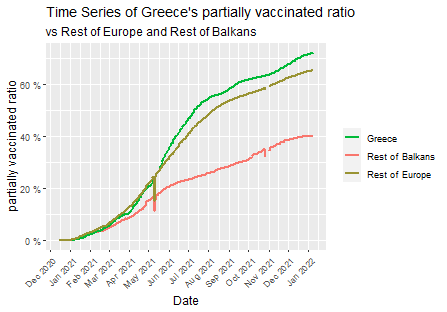
\includegraphics[width=12cm]{figures/Greece_vs_Europe_Balkans.png}
    \caption{Time Series partially vaccinated ratio of Greece vs rest of Europe and Balkans}
    \label{fig:greece_ratios}
\end{figure}
\FloatBarrier %fix position of image to its own subsection, not the next

As presented in \textbf{Figure \ref{fig:africa_ratios}}, Greece has stayed ahead of the average of the rest of European countries' partially vaccination ratio for most of the pandemic duration up until 08-01-2022 and has exceeded 70\% on that date.
\\
The rest of Balkans on average sit around 40\% and are way below the rest of European countries' ratio.

\section{Conclusions}
The vaccination performance of countries, group of countries and continents was examined over a time period or on the last day of dataset update, 08-01-2022. \\
On a continent level, South America is the leader in the administration of at least one vaccine dose whereas Africa comes last. In the latter, less populated countries have performed better than more populated ones, the majority of them scoring below 40\%. In Europe, Balkan counties are at the bottom of the vaccination chart, whereas northwestern countries are in the top positions. However, in the top 3 positions sit European south countries, Malta, Portugal, and Spain.\\
On a country level, a pattern of high vaccination rates was easier to spot on less populated countries. United Arab Emirates and Malta have topped the chart of vaccination rates, having vaccinated all their population with at least one dose. China seems to be an exception to this rule though being a top performer.
\\
Finally, Greece was compared to the rest of the European countries (excl. Greece) and the rest of Balkan countries (excl. Greece) and was found to perform above both averages for most of the time since the beginning of vaccination programs. Its vaccination ratio on 08-01-2022  for at least one vaccine dose sits over 70\% and therefore the country seems to be relatively safeguarded against the pandemic.